\documentclass[11pt]{beamer}
\usetheme{Rochester}
\usepackage[utf8]{inputenc}
\usepackage[francais]{babel}
\usepackage[T1]{fontenc}
\usepackage{amsmath}
\usepackage{amsfonts}
\usepackage{amssymb}
\usepackage{tikz}

\author{Brachet Matthieu}
\title{Les mathématiques de l'atmosphère}
\logo{iecl.jpg} 
\date[18.05.2016]{18 mai 2016} 
\begin{document}

\begin{frame}
\titlepage
\end{frame}

\begin{frame}{Parcours :}

\textbf{Brachet Matthieu}, né à Lille (59) en 1991.

\vspace{1cm}
\textbf{Parcours : }
\begin{itemize}
\item 2008 : Baccalauréat scientifique à Clermont de l'Oise (60), \pause
\item 2008 - 2010 : Classe préparatoires aux grandes écoles MPSI et MP à Compiègne (60), \pause
\item 2010 - 2014 : Université Picardie Jules Verne (Licence et Master en mathématiques appliquées) à Amiens (80), \pause
\item Aujourd'hui : Doctorant à l'Université de Lorraine (57). 
\end{itemize}

\end{frame}

%% *************************************************

\begin{frame}{Problème :}

\begin{block}{Ma thèse :}
Schémas compacts hermitiens sur la sphère - applications en climatologie et océanographie numérique
\end{block}

\begin{columns}
\column{0.45\textwidth}
\begin{block}{Motivations :}
Prédire les mouvements de l'atmosphère autour d'une planète.
\end{block}

\column{0.45\textwidth}
\begin{tikzpicture}[scale=0.7]
\draw [fill=gray!20] (0.9,1.3) circle (1.3) ;
\draw (0.9,2.2) node[below]{Maths.} ;
\draw (0,0) circle (1.2) ;
\draw (-0.5,0) node[below]{Info.} ;
\draw (1.8,0) circle (1.2) ;
\draw (2,0) node[below]{Phys.} ;
\end{tikzpicture}
\end{columns}
\end{frame}

%% *************************************************

\begin{frame}{Modélisation :}

\begin{columns}
\column{0.45\textwidth}
\begin{center}
\begin{figure}
\includegraphics[scale=0.5]{nenuphare.jpg}
\caption{\begin{tiny}Lac de Grand-Lieu - Crédit photo : J-M. Gillier / SNPN
\end{tiny} }
\end{figure}
\end{center}


\column{0.45\textwidth}
\begin{block}{Petite énigme}
Un nénuphar vit au milieu d'un étang, tous les jours sa surface double. Il a mis 17 jours pour recouvrir la moitié de la surface totale de l'étang. Combien de jours mettra ce même nénuphar pour recouvrir l'intégralité de la surface de l'étang ?
\end{block}

\pause
\begin{flushright}
Réponse : 18 jours.
\end{flushright}
\end{columns}

\end{frame}

\begin{frame}{Qu'est ce que l'on a fait ?}
\begin{block}{un modèle mathématique :}
$$S(\text{demain}) = 2 \times S(\text{aujourd'hui})$$
\end{block}

Questions supplémentaires :
\begin{itemize}
\item à 15 jours, 8 heures et 23 minutes?
\item Recouvrement des nénuphares?
\item Chien du voisin?
\end{itemize}

\begin{block}{Nouveau modèle : }
$$V(t) = \alpha(t) \times S(t) \times \left( 1 - \dfrac{S(t)}{S_{\text{étang}}} \right)$$
\end{block}

\end{frame}

\begin{frame}{Pour l'atmosphère :}

Quels paramètres ?
\begin{itemize}
\item Force de Coriolis,
\item Gravité,
\item Viscosité,
\item \'Epaisseur de l'atmosphère,
\item ...
\end{itemize}

\begin{block}{Mise en équations :}
\begin{equation*}
\left \{
\begin{array}{rcl}
\partial_t h + \nabla \cdot \left( h \mathbf{v} \right) & = & 0 \\
\partial_t ( h \mathbf{v} ) + \nabla \cdot \left( h \mathbf{v} \otimes \mathbf{v} + \dfrac{1}{2} g h^2 \mathbb{I}d \right) & = & - f \mathbf{k} \wedge \left( h \mathbf{v} \right)
\end{array}
\right.
\end{equation*}
\end{block}
\end{frame}

%% *************************************************

\begin{frame}{Constat :}
\begin{columns}
\column{0.52\textwidth}
\begin{block}{Nénuphare : }
$$V(t) = \alpha(t) \times S(t) \times \left( 1 - \dfrac{S(t)}{S_{\text{étang}}} \right)$$
\end{block}


\column{0.49\textwidth}
\begin{block}{Atmosphère :}
\begin{equation*}
\left \{
\begin{array}{rcl}
\partial_t h + \nabla \cdot \left( h \mathbf{v} \right) & = & 0 \\
\partial_t ( h \mathbf{v} ) + ... &  & 
\end{array}
\right.
\end{equation*}
\end{block}
\end{columns}

\begin{alertblock}{}
Comment je calcule la taille de mon nénuphare la dedans???
\end{alertblock}

\end{frame}

\begin{frame}
\begin{block}{}
Résolution par ordinateur
\end{block}

\begin{block}{Ordinateur :}
\begin{itemize}
\item mémoire finie : nombre fini de décimales,

\item pas de temps continu,

\item besoin de discrétiser.

\end{itemize}
\end{block}

\begin{block}{But :}
Méthode \textbf{rapide} et \textbf{précise}.

\end{block}

\end{frame}



\begin{frame}{Résolution numérique :}
\textbf{Approximation :}
$$V(t) = \dfrac{\text{Taille en plus}}{\text{temps nécessaire}}$$

Mathématiquement (méthode d'Euler Explicite) :

$$V(t) \approx \dfrac{S(t+\Delta t)-S(t)}{\Delta t} \approx \alpha(t) \times S(t) \times \left( 1 - \dfrac{S(t)}{S_{\text{étang}}} \right)$$

\end{frame}

\begin{frame}

$$S(\text{maintenant}) = S(\text{juste avant}) + \text{évolution}$$

\begin{center}
\begin{tikzpicture}[scale=1]
\draw [>=latex,->] (0,0) -- (8,0);
\draw (0,0) node[below] {0 sec} node{$\bullet$};
\draw (1.5,0) node[below] {5 sec} node{$\bullet$};
\draw (3,0) node[below] {10 sec} node{$\bullet$};
\draw (6,0) node[below] {1 h} node{$\bullet$};
\draw [>=latex,->] (1.5,0.2) arc (180:0:0.75) ;
\end{tikzpicture}
\end{center}

C'est la \textbf{discrétisation} (ici discrétisation en temps).

\end{frame}

\begin{frame}{Pour l'atmosphère :}

\begin{block}{Discrétisation}
\begin{itemize}
\item discrétisation en temps,
\item grillage sur la sphère.
\end{itemize}
\end{block}

\begin{figure}
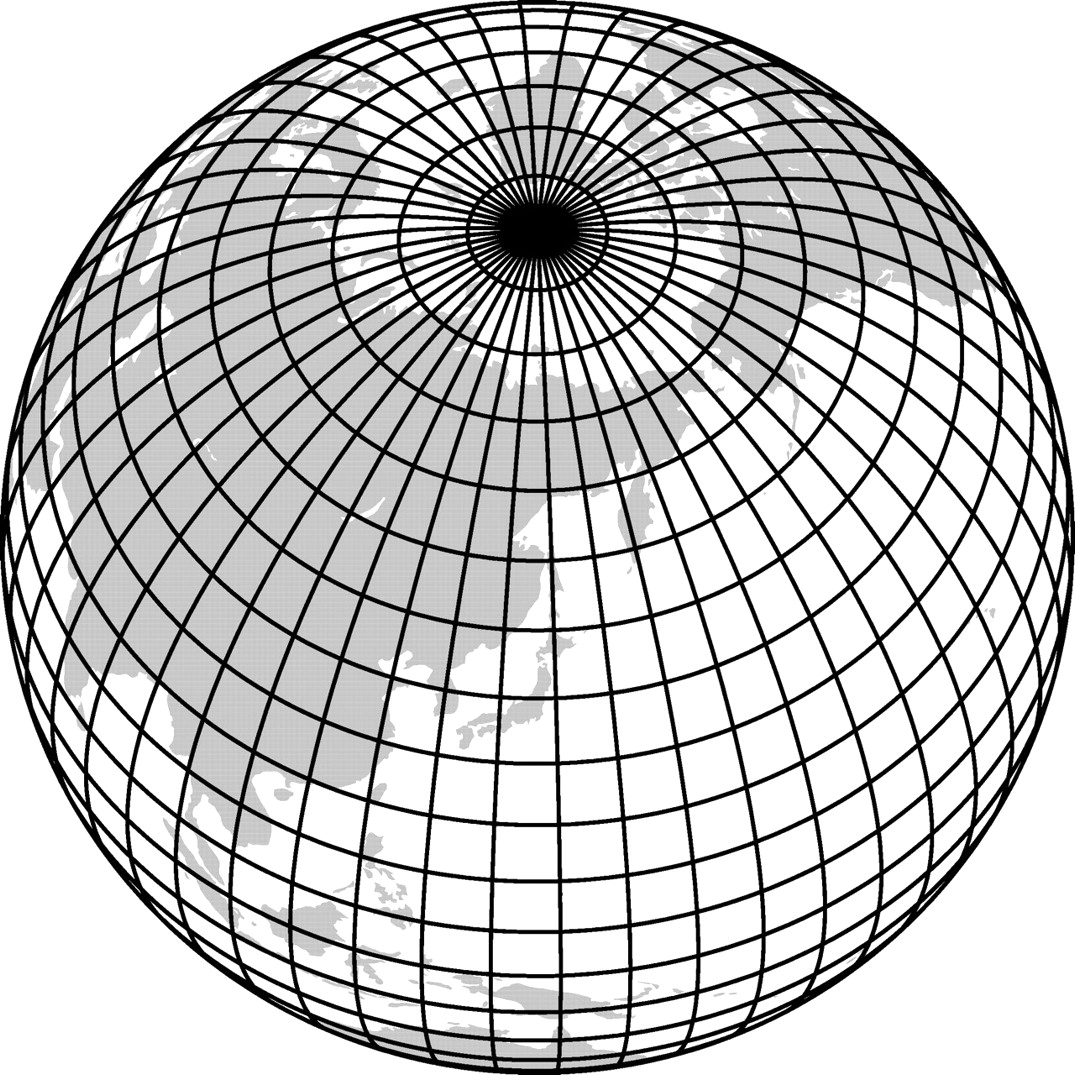
\includegraphics[height=3cm]{lonlat_grid.jpg} \hspace{1cm}
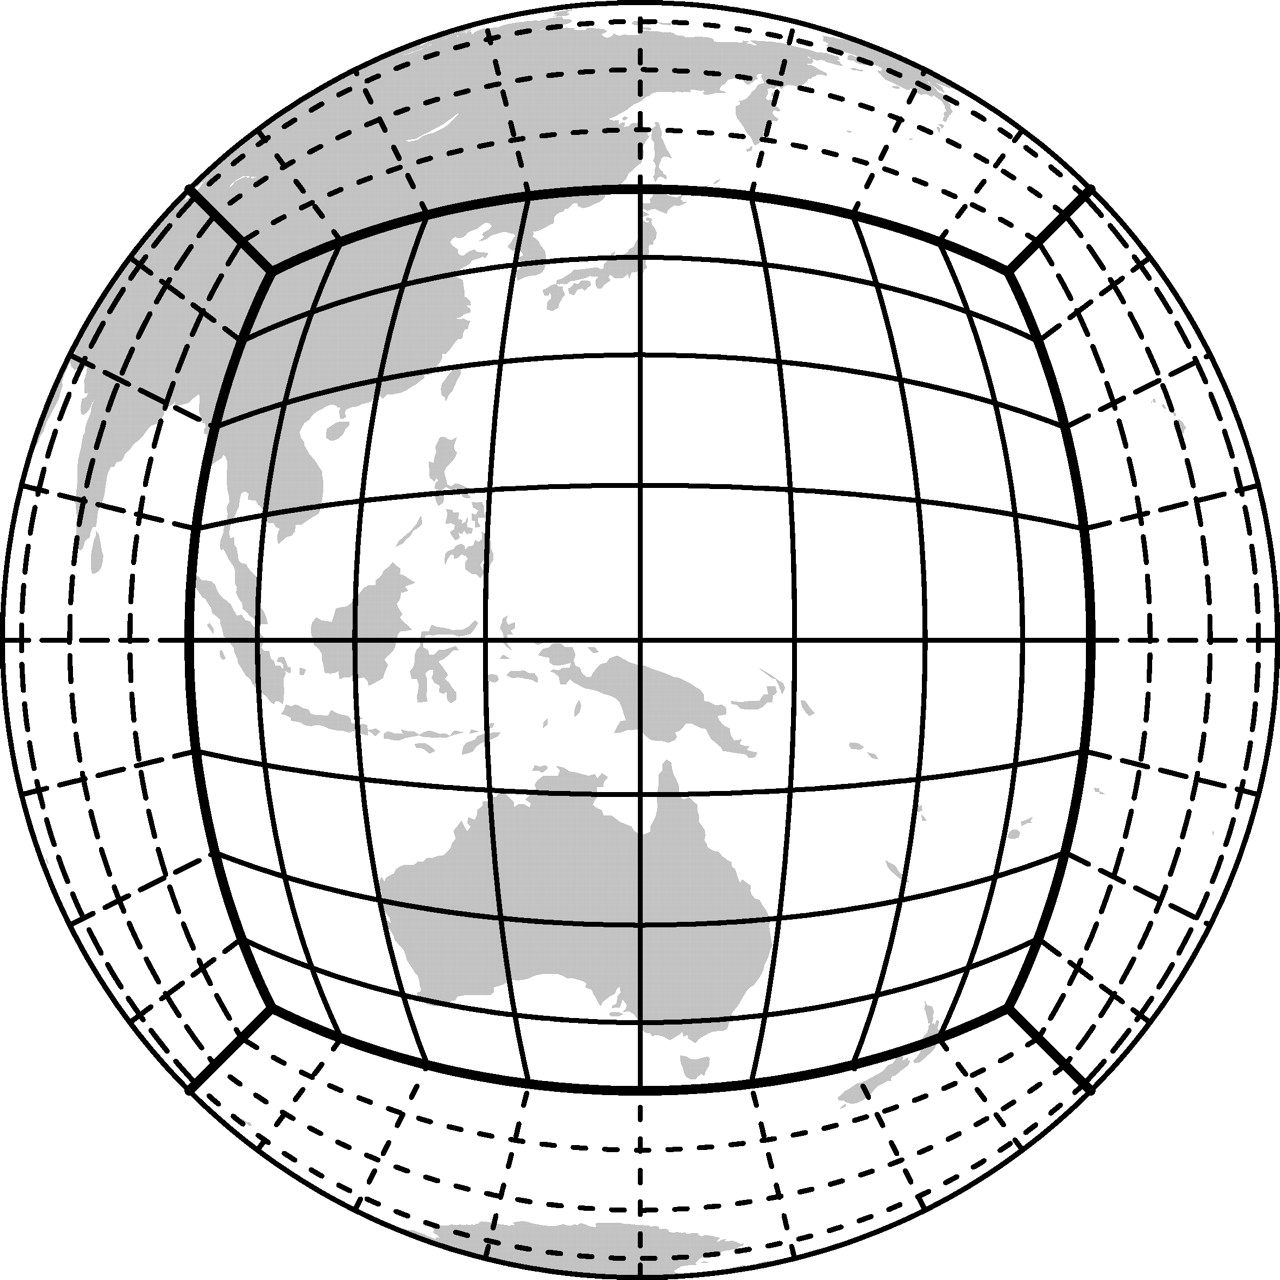
\includegraphics[height=3cm]{CS_grid.jpg}
\caption{Quelques maillages de la sphère}
\end{figure}

\end{frame}

\begin{frame}{Bilan :}
\begin{columns}
\column{0.45\textwidth}
\begin{block}{}
\begin{itemize}
\item Calcul de la solution aux "noeuds" du grillage,
\item Calcul à des temps fixés (nombreux).
\end{itemize}
\end{block}

\column{0.45\textwidth}
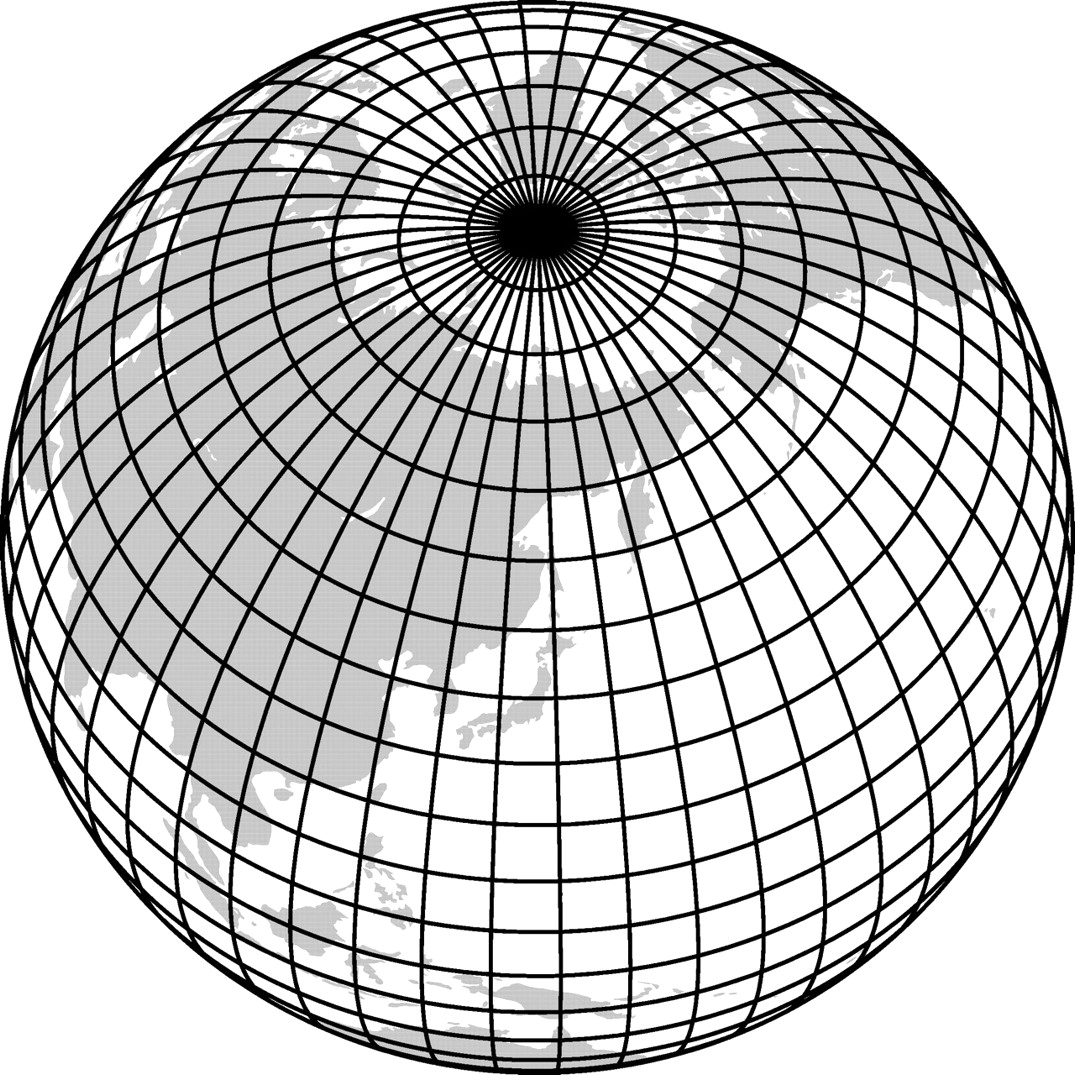
\includegraphics[height=3cm]{lonlat_grid.jpg} 

\end{columns}
\end{frame}


%% *************************************************

\begin{frame}{Validation :}
\begin{block}{}
Comment savoir si j'ai bien bossé?
\end{block}

\pause
\begin{itemize}
\item Comparaison avec la réalité?
\item Comparaison avec une formule?
\end{itemize}
\end{frame}

\begin{frame}{Comparaison avec la réalité}
\begin{block}{Idée :}
Comparer ce que donne la méthode numérique avec la réalité.

\vspace{0.3cm}
\begin{center}
\fbox{Réalité} $\longleftrightarrow$ \fbox{Méthode}
\end{center}
\vspace{0.3cm}
\end{block}

\begin{exampleblock}{}
Permet de savoir si on représente le bon phénomène.
\end{exampleblock}
\end{frame}


\begin{frame}{Comparaison avec une formule :}
$\Rightarrow$ Pour moi : pas de comparaison avec la réalité. C'est un autre niveau du travail !

Comparaison avec une solution exacte ?

$$V(t) = \alpha(t) \times S(t) \times \left( 1 - \dfrac{S(t)}{S_{\text{étang}}} \right)$$

Si $\alpha(t) = 1$, alors $S(t)$ connu à chaque instant.

\begin{exampleblock}{}
La différence entre la valeur exacte et la valeur approchée est-elle faible?
\end{exampleblock}

\end{frame}

\begin{frame}
\begin{figure}
\href{run:ref_7363864802_NSE.avi}{\includegraphics[height=4cm]{NS_ref_7363824432_omega.png}} 
\href{run:ref_7363145849_test_2.avi}{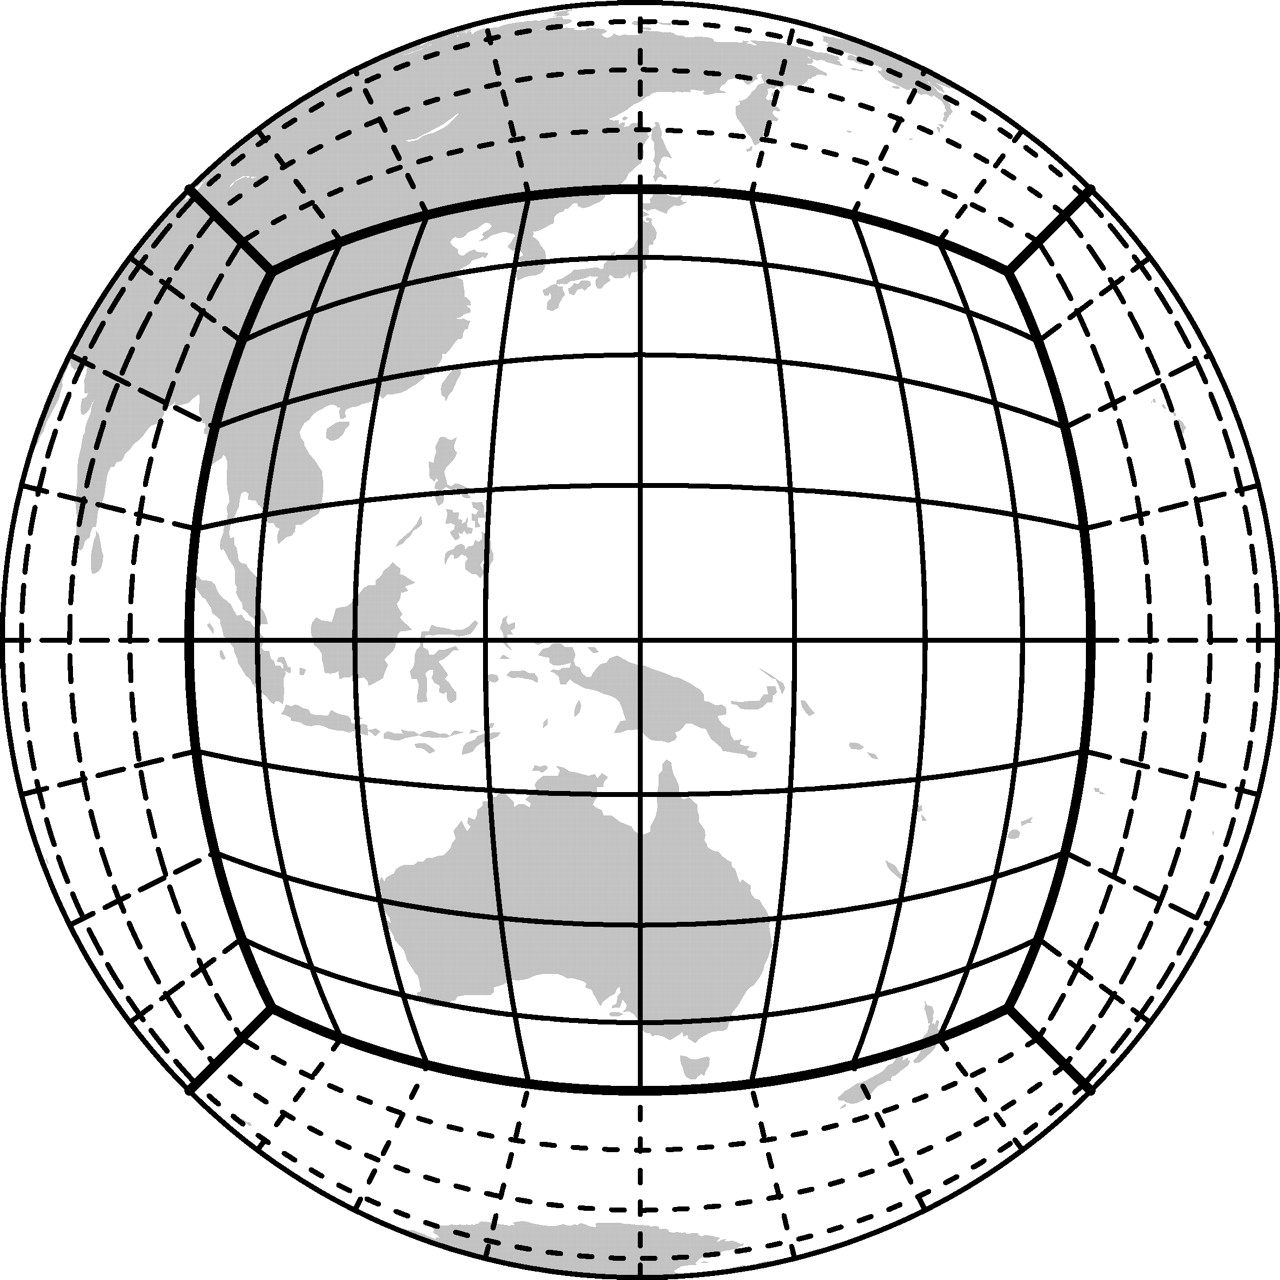
\includegraphics[height=4cm]{CS_grid.jpg}} 
\caption{Un test particulier}
\end{figure}
\end{frame}

\begin{frame}{A la fin...}
\begin{block}{Qu'a-t-on?}
\begin{itemize}
\item Equation sur un phénomène,
\item Méthode pour résoudre l'équation,
\item Validation.
\end{itemize}
\end{block}

\begin{block}{A présent}
Rendre l'équation de départ plus complète et recommencer.
\end{block}

\end{frame}


%% ************************************************************

\begin{frame}

\begin{block}{Autre énigme...}
Ce matin, plus de courant chez moi, obligé de m'habiller dans le noir.
Dans mon tiroir, 10 chaussettes blanches et autant de noires. 

Combien en prendre au minimum pour être sur d'en avoir deux de la même couleur?
\end{block}

\end{frame}


\begin{frame}
\begin{center}
Merci de votre attention. :)
\end{center}
\end{frame}



\end{document}